% Created 2016-04-18 Mon 21:44
\documentclass[11pt, a4paper]{article}
\usepackage[utf8]{inputenc}
\usepackage[T1]{fontenc}
\usepackage{fixltx2e}
\usepackage{graphicx}
\usepackage{longtable}
\usepackage{float}
\usepackage{wrapfig}
\usepackage{soul}
\usepackage{textcomp}
\usepackage{marvosym}
\usepackage{wasysym}
\usepackage{latexsym}
\usepackage{amssymb}
\usepackage{hyperref}
\tolerance=1000
\usepackage{minted}
\usepackage[utf8]{inputenc}
\usepackage[english]{babel}
\usepackage{graphicx}
\usepackage[left=2.35cm, right=3.35cm, top=3.35cm, bottom=3.0cm]{geometry}
\usepackage{titling}
\providecommand{\alert}[1]{\textbf{#1}}

\title{Statistical methods for bioinformatics \linebreak Model selection and regularization}
\author{Cedric Lood}
\date{\today}
\hypersetup{
  pdfkeywords={},
  pdfsubject={},
  pdfcreator={Emacs Org-mode version 7.9.3f}}

\begin{document}

\maketitle


\graphicspath{ {figures/} }
\setlength{\droptitle}{-5em} 
\setlength{\parindent}{0cm}

\section{Conceptual exercises}
\label{sec-1}
\subsection{Question 5}
\label{sec-1-1}
\subsubsection{Part a}
\label{sec-1-1-1}

We want to minimize the ridge regression defined by $RSS + \lambda \sum\limits_{i=1}^p \hat{\beta}_i^2$

\begin{itemize}
\item $min\Big[\sum\limits_{i=1}^n {(y_i - \hat{\beta}_0 - \sum\limits_{j=1}^p {\hat{\beta}_jx_j} )^2} + \lambda \sum\limits_{i=1}^p \hat{\beta}_i^2\Big]$
\item we have as constraints that $\hat{\beta}_0 = 0, p=2$, hence we can
  reformulate the optimisation as $min\Big[\sum\limits_{i=1}^n {(y_i - \sum\limits_{j=1}^2 {\hat{\beta}_jx_j} )^2} + \lambda \sum\limits_{i=1}^2 \hat{\beta}_i^2\Big]$
\item which can be expanded into $min\Big[ (y_1 - \hat{\beta}_1x_{11} - \hat{\beta}_2x_{12})^2 + (y_2 - \hat{\beta}_1x_{21} - \hat{\beta}_2x_{22})^2 + \lambda (\hat{\beta}_1^2 + \hat{\beta}_2^2)\Big]$
\end{itemize}
\subsubsection{Part b}
\label{sec-1-1-2}

For this, we can simply take the derivatives of the ridge regression
with respect to $\hat{\beta}_1$ and $\hat{\beta}_2$.
\subsubsection{Part c}
\label{sec-1-1-3}

Very similar to part a, the only difference between the lasso method
and the ridge regression lies with the norm taken of the
parameters. Lasso used a first-order norm (L1):

$min\Big[ (y_1 - \hat{\beta}_1x_{11} - \hat{\beta}_2x_{12})^2 + (y_2 - \hat{\beta}_1x_{21} - \hat{\beta}_2x_{22})^2 + \lambda (|\hat{\beta}_1| + |\hat{\beta}_2|)\Big]$
\subsubsection{Part d}
\label{sec-1-1-4}

skipped
\section{Applied exercises}
\label{sec-2}


Here is a list of libraries I used for the 2 exercises:

\begin{minted}[]{R}
library(ggplot2)
library(gridExtra)
library(leaps)
library(glmnet)
options(digits = 2)
\end{minted}
\subsection{Question 8}
\label{sec-2-1}
\subsubsection{Part a, b}
\label{sec-2-1-1}


\begin{minted}[]{R}
## part a: simulated dataset creation
set.seed(1)
x <- rnorm(100)
noise <- rnorm(100)
x_true <- seq(-3.0,3.0,0.01)

## part b: response vector with given model y = 1x^3 - 2x^2 + 3x + 5
y <- 2*x^3 + 0.5*x^2 + 3*x + 5 + noise
f <- 2*x_true^3 + 0.5*x_true^2 + 3*x_true+ 5

p1 <- qplot(x,y)
p2 <- qplot(x_true,f, geom="line")
grid.arrange(p1, p2, ncol=2)
ggsave("fun.pdf", arrangeGrob(p1, p2, ncol = 2), width = 16, height = 8, units = "cm")
\end{minted}

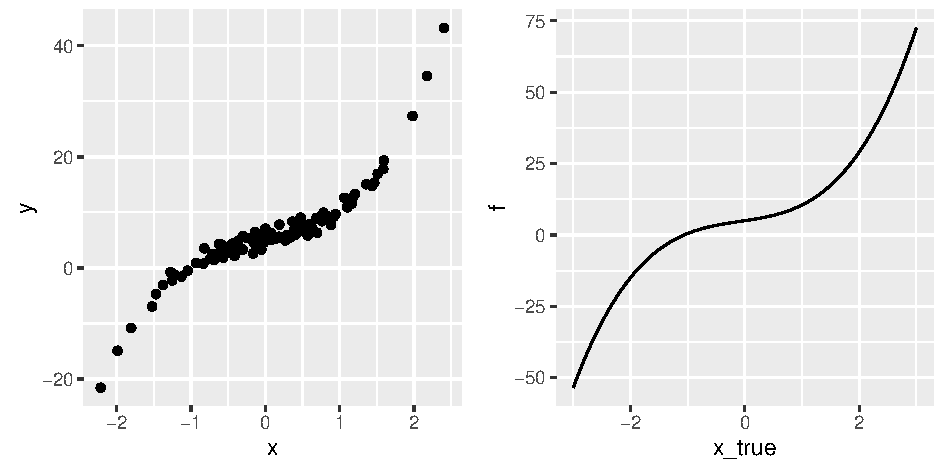
\includegraphics[scale=1]{fun.pdf}
\subsubsection{Part c}
\label{sec-2-1-2}


\begin{minted}[]{R}
## part c: perform best subset selection
dataset <- data.frame(x, y)
regfit.full <- regsubsets(y ~ poly(x, 10, raw = TRUE), data = dataset, nvmax = 10)
regfit.summary <- summary(regfit.full)
which.min(regfit.summary$cp)
which.min(regfit.summary$bic)
which.max(regfit.summary$adjr2)

# plotting results
cp <- qplot(1:10, regfit.summary$cp, geom="line") +
    xlab("Polynomial degree") + ylab("Cp") + scale_x_continuous(breaks=seq(1,10,1)) +
    geom_point(aes(x=4,y=regfit.summary$cp[4]),colour=I("sienna1"),size=3)

adjr2 <- qplot(1:10, regfit.summary$adjr2, geom="line") +
    xlab("Polynomial degree") + ylab("Adj-Rsquared") + scale_x_continuous(breaks=seq(1,10,1)) +
    geom_point(aes(x=4,y=regfit.summary$adjr2[4]),colour=I("sienna1"),size=3)

bic <- qplot(1:10, regfit.summary$bic, geom="line") +
    xlab("Polynomial degree") + ylab("BIC") + scale_x_continuous(breaks=seq(1,10,1)) +
    geom_point(aes(x=3,y=regfit.summary$bic[3]),colour=I("sienna1"),size=3)

grid.arrange(cp, adjr2, bic, ncol=2, nrow=2)
ggsave("BIC-AR2-Cp.pdf", arrangeGrob(cp, adjr2, bic, ncol = 2, nrow=2), )

coefficients(regfit.full, id = 3)
coefficients(regfit.full, id = 4)
\end{minted}

Here is the summary of the coefficients for the models that include 3
and 4 predictors:


\begin{verbatim}
> coefficients(regfit.full, id = 3)
          (Intercept) poly(x, 10, raw = T)1 poly(x, 10, raw = T)3 
                5.192                 3.043                 1.985 
poly(x, 10, raw = T)4 
                0.089 
> sort(x)  C-c C-c
> coefficients(regfit.full, id = 4)
          (Intercept) poly(x, 10, raw = T)1 poly(x, 10, raw = T)2 
                5.072                 3.387                 0.346 
poly(x, 10, raw = T)3 poly(x, 10, raw = T)5 
                1.558                 0.081
\end{verbatim}

The graphs, which upon visual inspection allows to decide which model
to use indicate 2 different optimal choices. 3 and 4 predictors. Note
that the most convincing graph seems to be the one using the
\emph{BIC} criterion. The others have a minimum at 4, but that minimum
is very close to that located at 3.

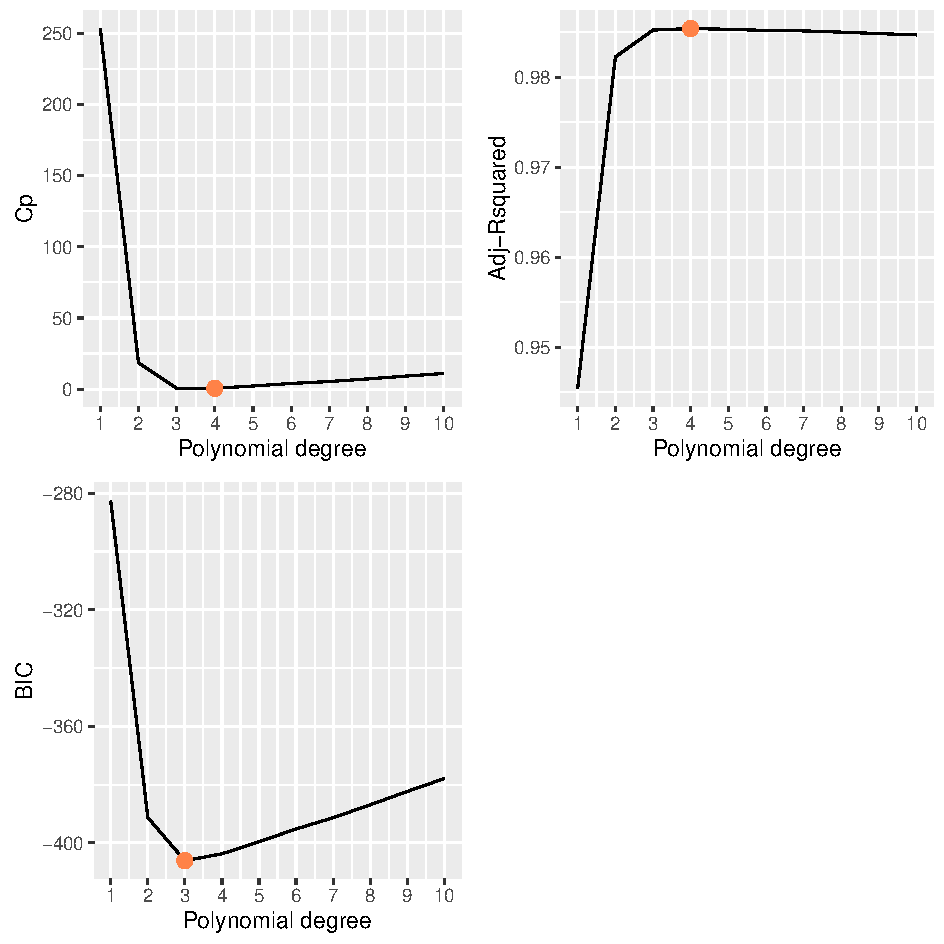
\includegraphics[scale=1]{BIC-AR2-Cp.pdf}


\begin{minted}[]{R}
## Forward selection
regfit.fwd <- regsubsets(y ~ poly(x, 10, raw = TRUE), data = dataset, nvmax = 10, method = "forward")
fwd.summary <-  summary(regfit.fwd)
which.min(fwd.summary$cp)
which.max(fwd.summary$adjr2)
which.min(fwd.summary$bic)

cp <- qplot(1:10, fwd.summary$cp, geom="line") +
    xlab("Polynomial degree") + ylab("Cp") + scale_x_continuous(breaks=seq(1,10,1)) +
    geom_point(aes(x=3,y=fwd.summary$cp[3]),colour=I("sienna1"),size=3)

adjr2 <- qplot(1:10, fwd.summary$adjr2, geom="line") +
    xlab("Polynomial degree") + ylab("Adj-Rsquared") + scale_x_continuous(breaks=seq(1,10,1)) +
    geom_point(aes(x=4,y=fwd.summary$adjr2[4]),colour=I("sienna1"),size=3)

bic <- qplot(1:10, fwd.summary$bic, geom="line") +
    xlab("Polynomial degree") + ylab("BIC") + scale_x_continuous(breaks=seq(1,10,1)) +
    geom_point(aes(x=3,y=fwd.summary$bic[3]),colour=I("sienna1"),size=3)

grid.arrange(cp, adjr2, bic, ncol=2, nrow=2)
ggsave("Fwd-BIC-AR2-Cp.pdf", arrangeGrob(cp, adjr2, bic, ncol = 2, nrow=2))
\end{minted}

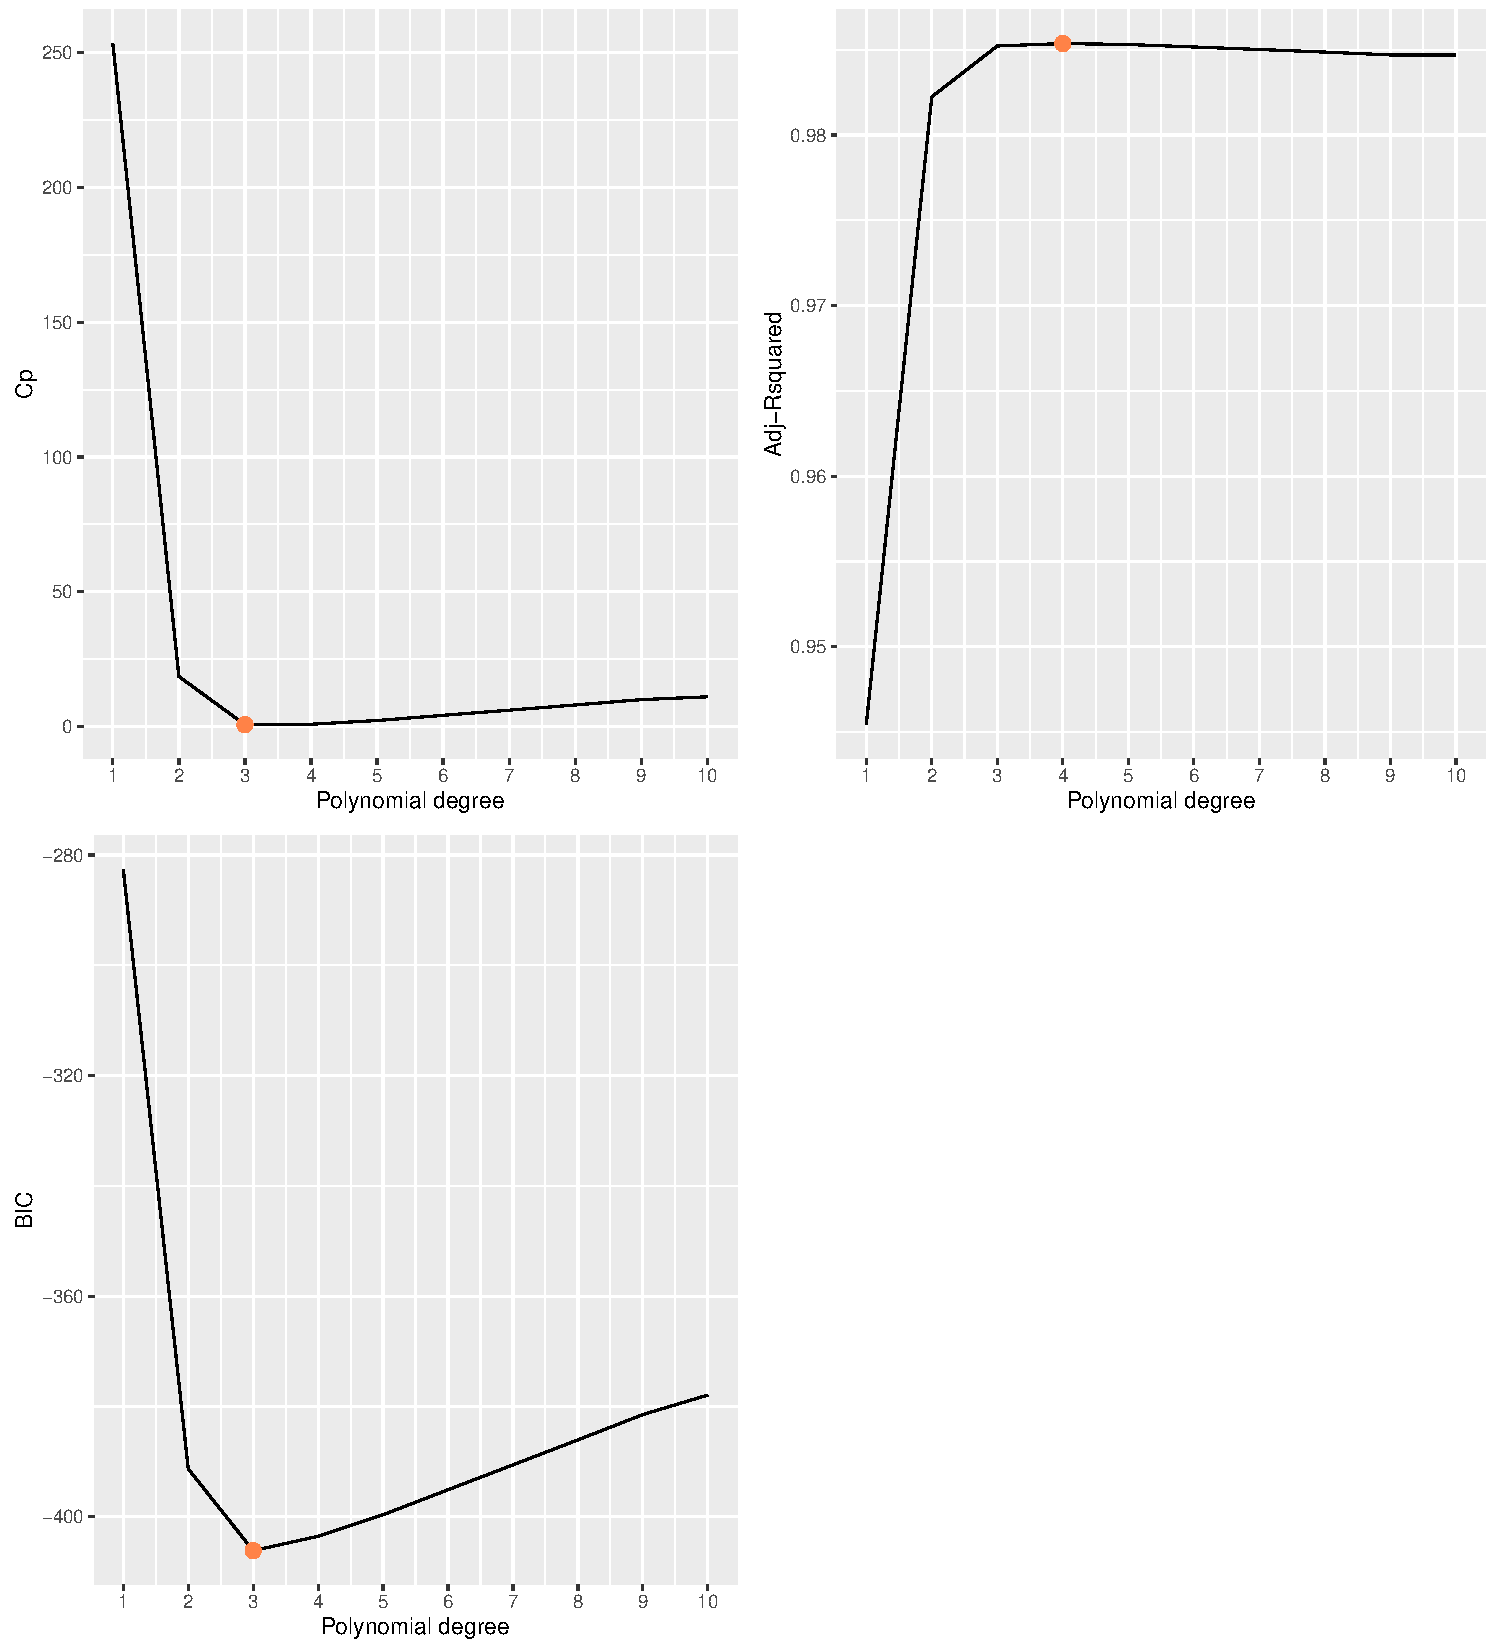
\includegraphics[scale=0.55]{Fwd-BIC-AR2-Cp.pdf}
\subsubsection{Part d}
\label{sec-2-1-3}


\begin{minted}[]{R}
## Backward selection
regfit.bwd <- regsubsets(y ~ poly(x, 10, raw = TRUE), data = dataset, nvmax = 10, method = "backward")
bwd.summary <-  summary(regfit.bwd)

which.min(bwd.summary$cp)
which.max(bwd.summary$adjr2)
which.min(bwd.summary$bic)

cp <- qplot(1:10, bwd.summary$cp, geom="line") +
    xlab("Polynomial degree") + ylab("Cp") + scale_x_continuous(breaks=seq(1,10,1)) +
    geom_point(aes(x=3,y=bwd.summary$cp[3]),colour=I("sienna1"),size=3)

adjr2 <- qplot(1:10, bwd.summary$adjr2, geom="line") +
    xlab("Polynomial degree") + ylab("Adj-Rsquared") + scale_x_continuous(breaks=seq(1,10,1)) +
    geom_point(aes(x=5,y=bwd.summary$adjr2[5]),colour=I("sienna1"),size=3)

bic <- qplot(1:10, bwd.summary$bic, geom="line") +
    xlab("Polynomial degree") + ylab("BIC") + scale_x_continuous(breaks=seq(1,10,1)) +
    geom_point(aes(x=3,y=bwd.summary$bic[3]),colour=I("sienna1"),size=3)

grid.arrange(cp, adjr2, bic, ncol=2, nrow=2)
ggsave("Bwd-BIC-AR2-Cp.pdf", arrangeGrob(cp, adjr2, bic, ncol = 2, nrow=2))
\end{minted}

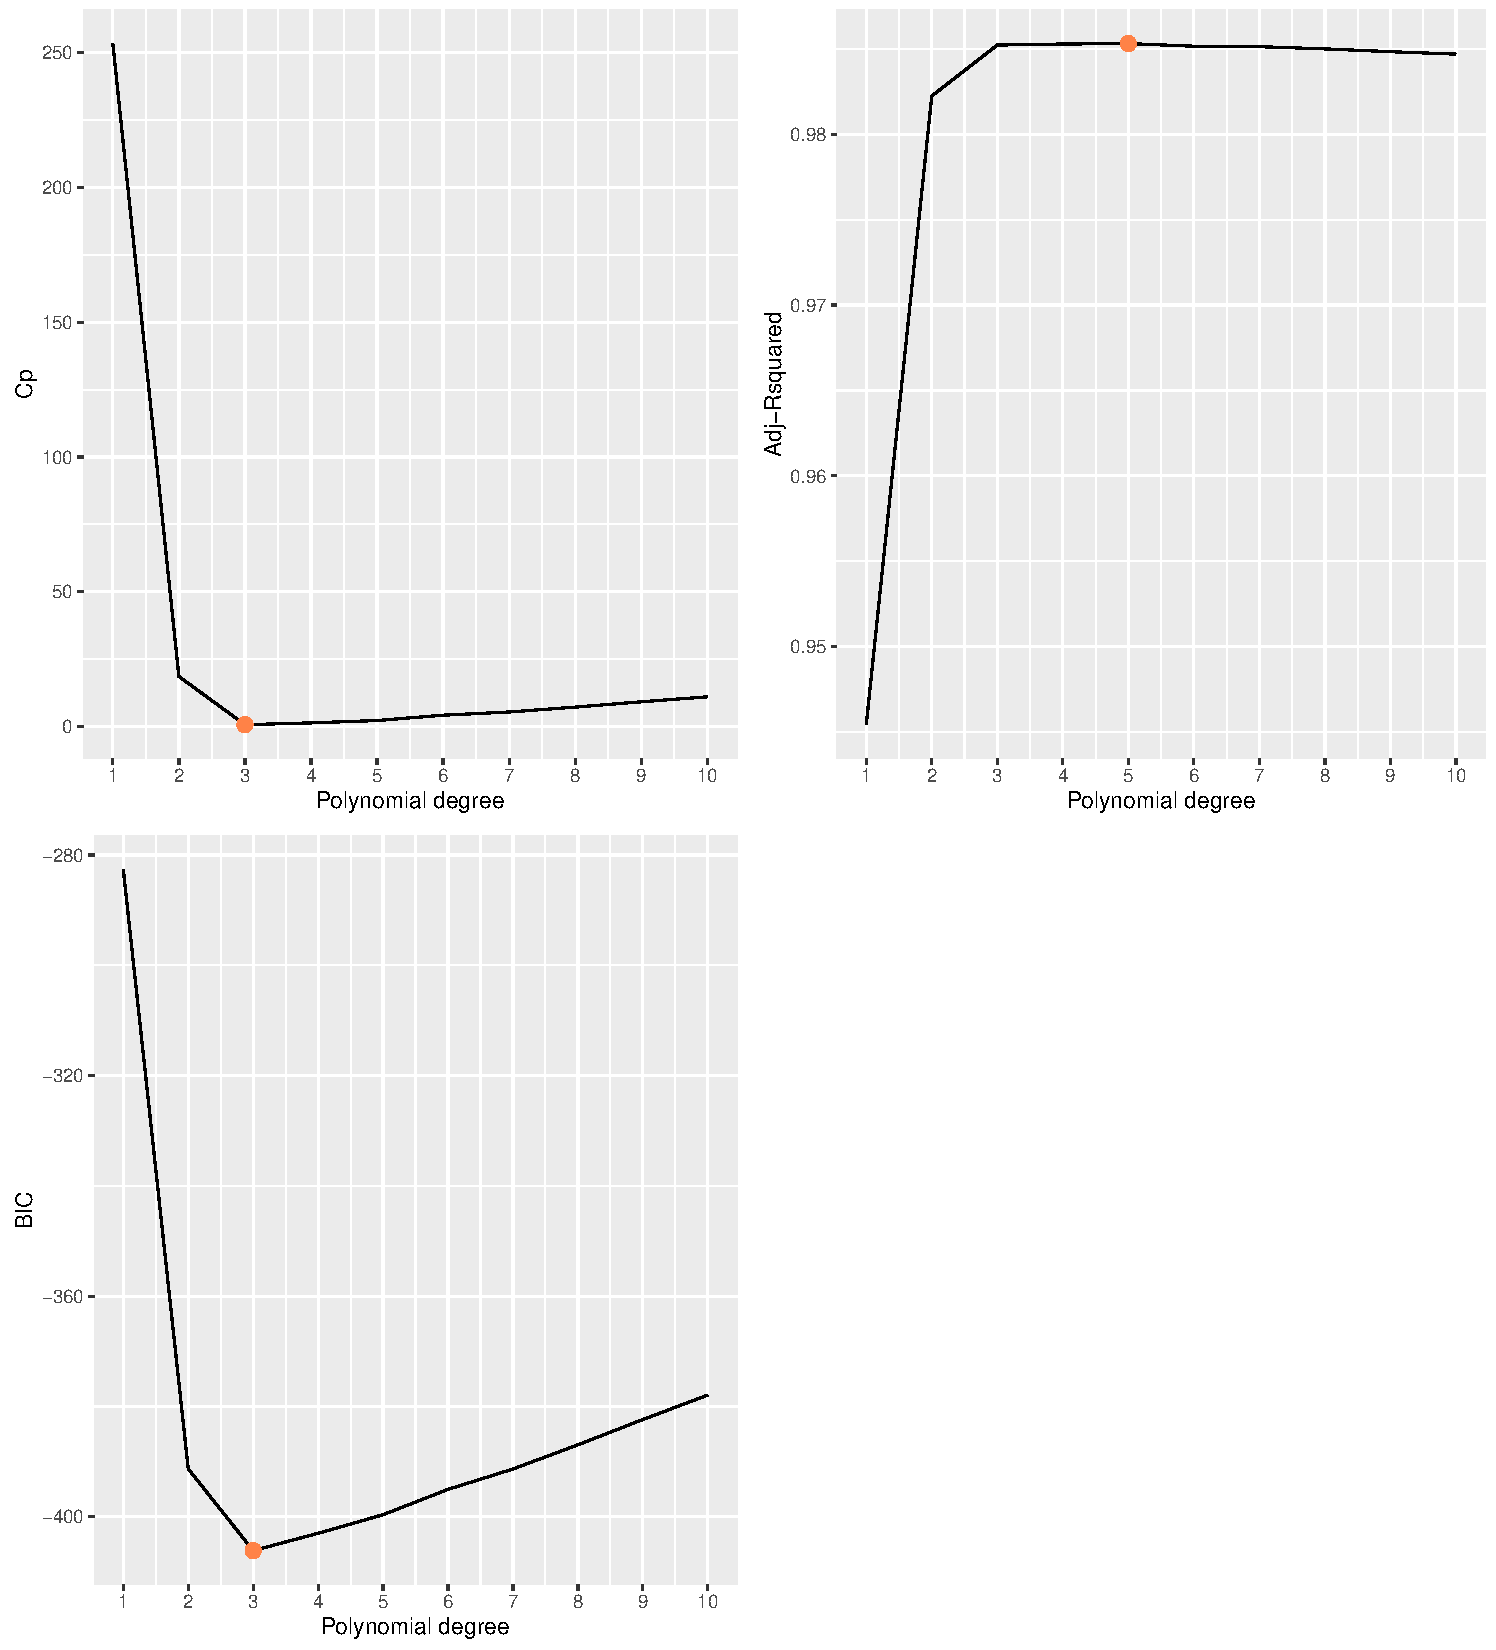
\includegraphics[scale=0.55]{Bwd-BIC-AR2-Cp.pdf}
\subsubsection{Part e}
\label{sec-2-1-4}


\begin{minted}[]{R}
xmat <- model.matrix(y ~ poly(x, 10, raw = T), data = dataset)[, -1]
lasso.mod <- cv.glmnet(xmat, y, alpha = 1)
best.lambda <- lasso.mod$lambda.min

pdf("lasso-plot.pdf", width=8, height=8)
plot(lasso.mod)
dev.off()

# Next fit the model on entire data using best lambda
best.model <- glmnet(xmat, y, alpha = 1)
predict(best.model, s = best.lambda, type = "coefficients")
\end{minted}

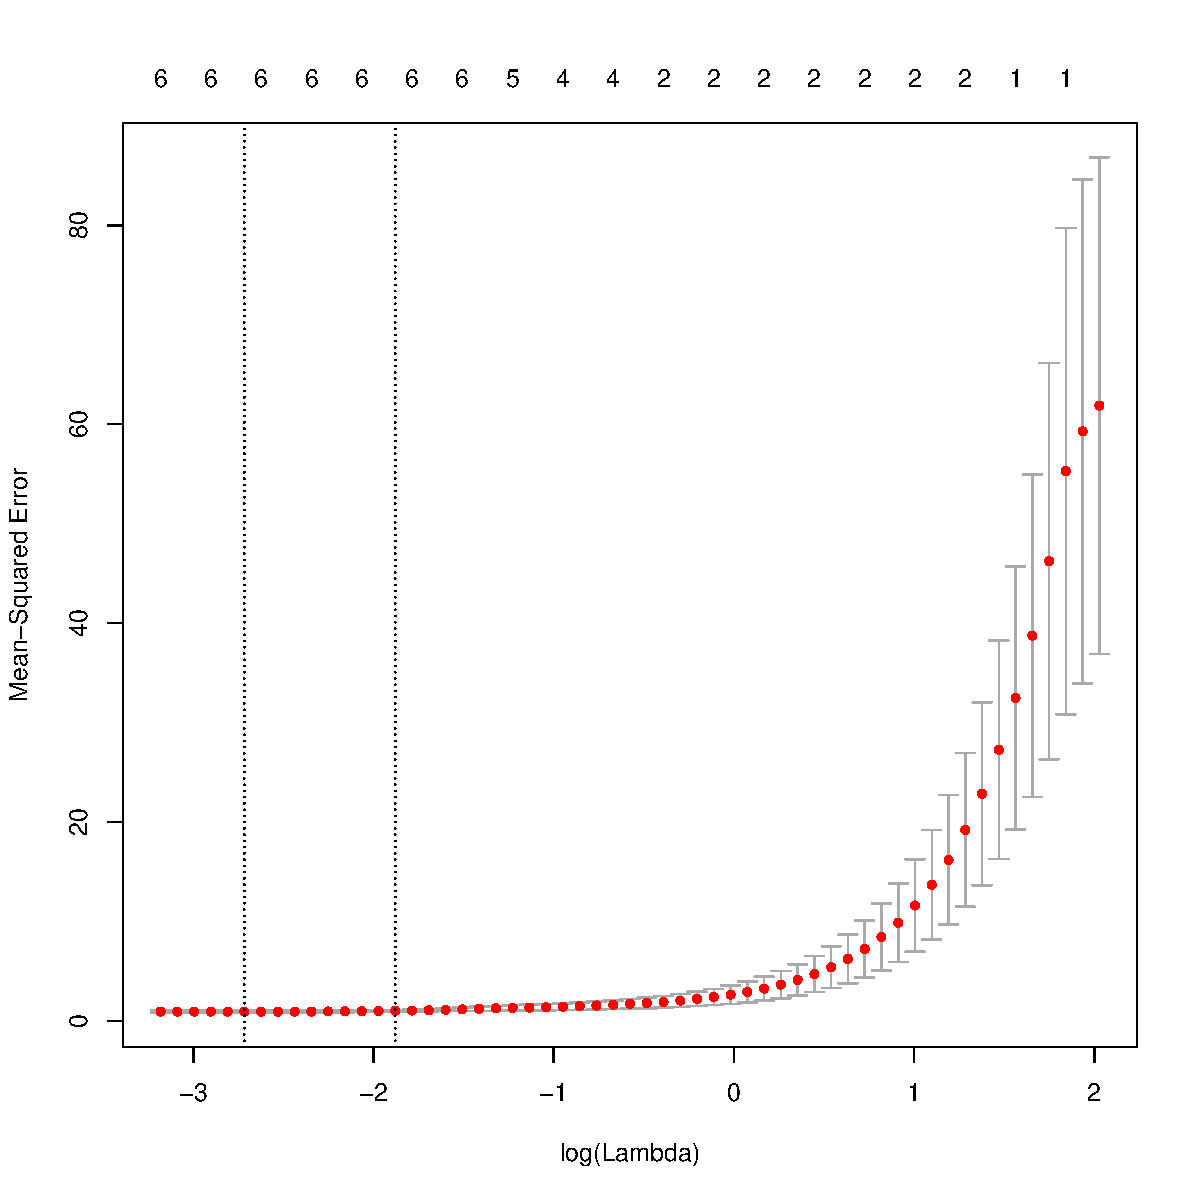
\includegraphics[scale=0.55]{lasso-plot.pdf}


\begin{verbatim}
> predict(best.model, s = best.lambda, type = "coefficients")
11 x 1 sparse Matrix of class "dgCMatrix"
                            1
(Intercept)            5.1776
poly(x, 10, raw = T)1  3.1552
poly(x, 10, raw = T)2  0.1273
poly(x, 10, raw = T)3  1.8183
poly(x, 10, raw = T)4  0.0422
poly(x, 10, raw = T)5  0.0032
poly(x, 10, raw = T)6  .     
poly(x, 10, raw = T)7  0.0054
poly(x, 10, raw = T)8  .     
poly(x, 10, raw = T)9  .     
poly(x, 10, raw = T)10 .
\end{verbatim}
\subsubsection{Part f}
\label{sec-2-1-5}

For this exercise, I used the following underlying function, with
Gaussian noise:


\begin{minted}[]{R}
y <- 5 + 2*x^7 + noise
dataset <- data.frame(x, y)
\end{minted}

Here is the best subset approach:


\begin{minted}[]{R}
## Best subset
regfit.full <- regsubsets(y ~ poly(x, 10, raw = TRUE), data = dataset, nvmax = 10)
regfit.summary <- summary(regfit.full)
which.min(regfit.summary$cp)
which.min(regfit.summary$bic)
which.max(regfit.summary$adjr2)

# plotting results best subset
cp <- qplot(1:10, regfit.summary$cp, geom="line") +
    xlab("Polynomial degree") + ylab("Cp") + scale_x_continuous(breaks=seq(1,10,1)) +
    geom_point(aes(x=2,y=regfit.summary$cp[2]),colour=I("sienna1"),size=3)

adjr2 <- qplot(1:10, regfit.summary$adjr2, geom="line") +
    xlab("Polynomial degree") + ylab("Adj-Rsquared") + scale_x_continuous(breaks=seq(1,10,1)) +
    geom_point(aes(x=4,y=regfit.summary$adjr2[4]),colour=I("sienna1"),size=3)

bic <- qplot(1:10, regfit.summary$bic, geom="line") +
    xlab("Polynomial degree") + ylab("BIC") + scale_x_continuous(breaks=seq(1,10,1)) +
    geom_point(aes(x=1,y=regfit.summary$bic[1]),colour=I("sienna1"),size=3)

grid.arrange(cp, adjr2, bic, ncol=2, nrow=2)
ggsave("BIC-AR2-Cp-f.pdf", arrangeGrob(cp, adjr2, bic, ncol = 2, nrow=2),
       width = 16, height = 16, units = "cm")
\end{minted}

\includegraphics[scale=0.55]{BIC-AR2-Cp-f.pdf.pdf}

And the lasso approach:


\begin{minted}[]{R}
## Lasso
xmat <- model.matrix(y ~ poly(x, 10, raw = T), data = dataset)[, -1]
lasso.mod <- cv.glmnet(xmat, y, alpha = 1)
best.lambda <- lasso.mod$lambda.min

best.model <- glmnet(xmat, y, alpha = 1)
predict(best.model, s = best.lambda, type = "coefficients")

pdf("lasso-plot-f.pdf", width=8, height=8)
plot(lasso.mod)
dev.off()
\end{minted}

\includegraphics[scale=.5]{lasso-plot-f.pdf}

As shown below for the coefficients, the lasso model is really spot on
when considering the underlying model used to generate the dataset.

\begin{verbatim}
> predict(best.model, s = best.lambda, type = "coefficients")
11 x 1 sparse Matrix of class "dgCMatrix"
                         1
(Intercept)            5.2
poly(x, 10, raw = T)1  .  
poly(x, 10, raw = T)2  .  
poly(x, 10, raw = T)3  .  
poly(x, 10, raw = T)4  .  
poly(x, 10, raw = T)5  .  
poly(x, 10, raw = T)6  .  
poly(x, 10, raw = T)7  1.9
poly(x, 10, raw = T)8  .  
poly(x, 10, raw = T)9  .  
poly(x, 10, raw = T)10 .
\end{verbatim}

\end{document}
